\section{倒易基矢量}
搞清楚倒易基矢量是什么以及它们如何简化对象显然在二维空间中最容易做到。给出一组基矢量$\left\{ \bb{g}_1,\bb{g}_2 \right\} $,我们如前文所述将点积$\bb{u}\cdot \bb{v}$的第一个矢量表示为$\bb{u}=u^1\bb{g}_1+u^2\bb{g}_2$。(在这个二维的例子中,点积的表达式足够短,我们不需要用到求和约定)不过,我们这里用一个新的(尚且未知的)基底$\left\{ \boldsymbol{g}^1,\boldsymbol{g}^2 \right\} $表述第二个矢量,写作$\boldsymbol{v}=v_1\boldsymbol{g}^1+v_2\boldsymbol{g}^2$,那么
\begin{align*}
	\bb{u}\cdot \bb{v}&=\left( u^1\bb{g}_1+u^2\bb{g}_2 \right) \cdot \left( v_1\bb{g}^1+v_2\bb{g}^2 \right)\\
	&=u^1v_1\bb{g}_1\cdot \bb{g}^1+u^1v_2\bb{g}_1\cdot \bb{g}^2+u^2v_1\bb{g}_2\cdot \bb{g}^1+u^2v_2\bb{g}_2\cdot \bb{g}^2
\end{align*}
我们的想法是提出$\bb{g}^1$和$\bb{g}^2$,这样上面的表达式可以简化为
\begin{equation*}
    \bb{u}\cdot \bb{v}=u^1v_1+u^2v_2
\end{equation*}
因此我们要求$\bb{g}_1\cdot \bb{g}^1=\bb{g}_2\cdot \bb{g}^2=1$以及$\bb{g}_1\cdot \bb{g}^2=\bb{g}_2\cdot \bb{g}^1=0$。给出$\bb{g}_1$和$\bb{g}_2$,我们可以如下用几何方法构造$\bb{g}_1$和$\bb{g}_2$:

如图\eqref{fig:2.3}a所示,作一条直线垂直于$\bb{g}_2$。因为$\bb{g}^1\cdot \bb{g}_2=0$,$\bb{g}^1$必然躺在这条直线上。现在,调整$\bb{g}^1$的方向和长度使$\bb{g}^1\cdot \bb{g}_1=1$,正如\eqref{fig:2.3}b所示。同理,我们可以构造$\bb{g}^2$。

\begin{figure}[htbp]
	\centering
	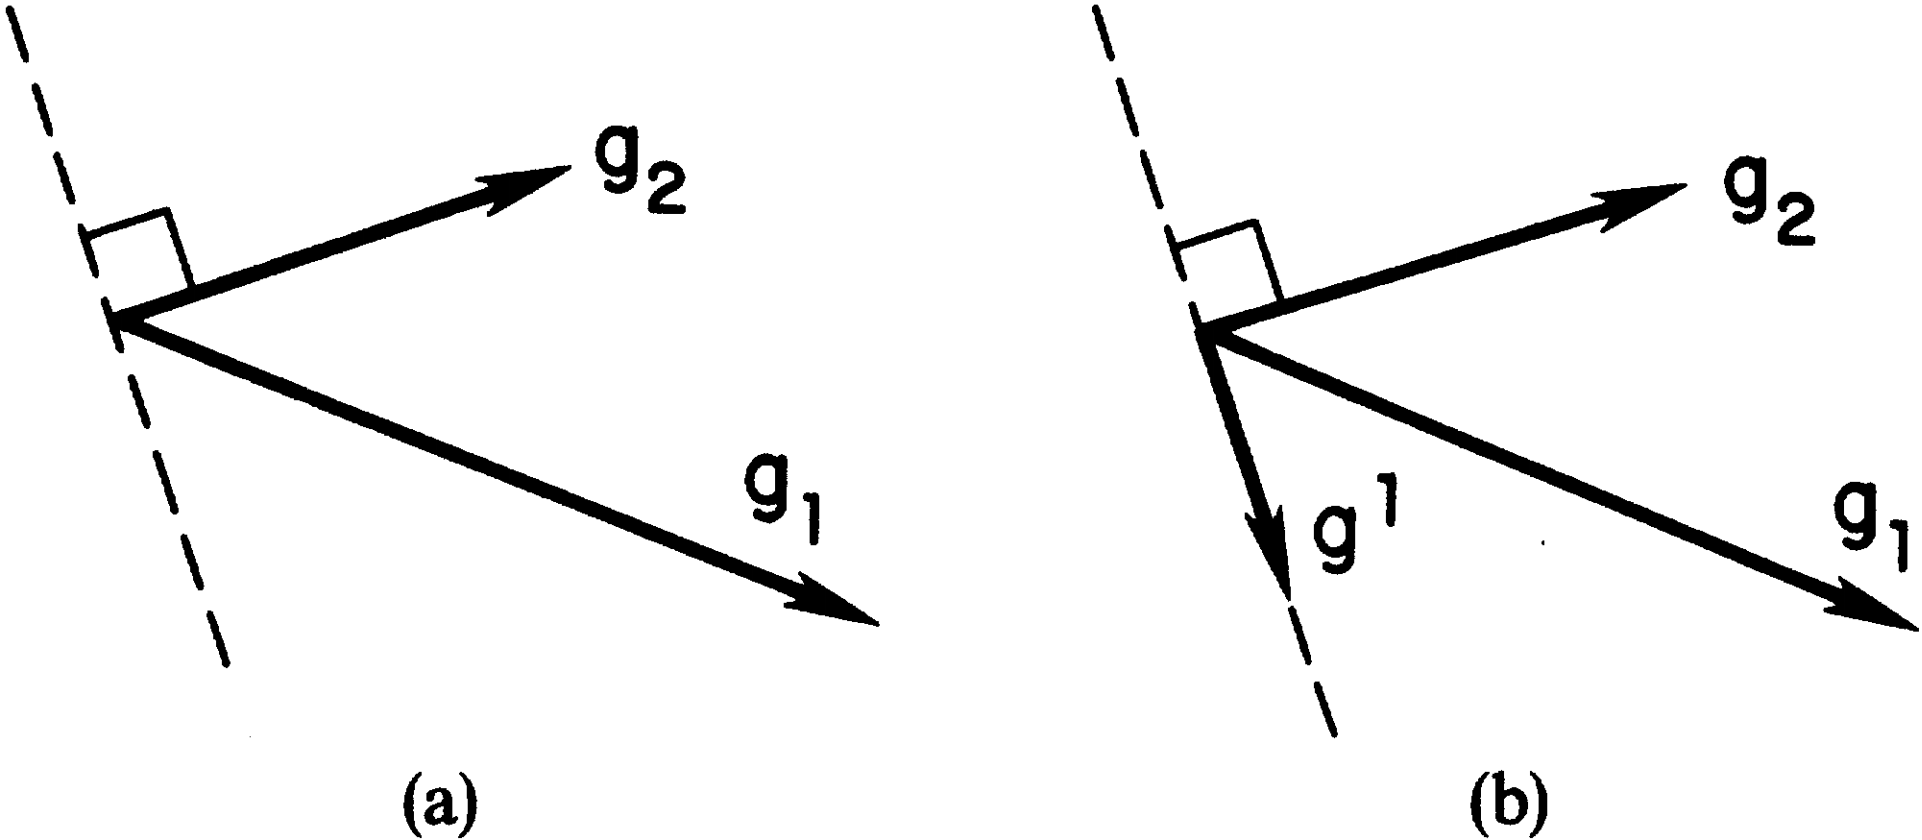
\includegraphics[width=0.65\textwidth]{./image/2.3.png}
	\caption{}
	\label{fig:2.3}
\end{figure}

基于对几何学的充分理解(尤其是在完成练习2.22之后),我们现在开发一种(计算机可以使用的)代数方法来构建n维的倒易基矢量。这将让我们在回到简化式\eqref{equ:2.3}的分量形式的问题之前绕一点弯路。

取$\left\{ \bb{g}_1,\bb{g}_2,\dots \right\} =\left\{ \bb{g}_j \right\} $为一组基底。那么,它就满足$G\ne 0$。回忆矩阵有关知识,我们可以知道$G^{-1}$存在。$G^{-1}$的第$i$列元素可视作矢量$\bb{g}^i$的笛卡尔坐标,其余皆类此,
\begin{equation*}
    G^{-1}=\left[ \begin{array}{c}
        \bb{g}^1\\
        \bb{g}^2\\
        \vdots\\
    \end{array} \right] =\left[ \bb{g}^1\begin{matrix}
        \bb{g}^2&		\cdots\\
    \end{matrix} \right] ^{\mathrm{T}}=\left[ \bb{g}^i \right] 
\end{equation*}
其中,$\mathrm{T}$表示转置。(当我们希望将$G$视为列向量的集合时,我们可以设$G=[\bb{g}_j]$以保持上述符号一致。)矩阵乘法法则规定,$G^{-1}G$的第$i$行,第$j$列元素是$G^{-1}$的第$i$行所有元素与$G$的第$j$列所有元素一一对应后的乘积之和。因此,$G^{-1}G=I$等价于
\begin{equation}\label{equ:2.4}
    \bb{g}^i\cdot \bb{g}_j=\delta _{j}^{i}=\left\{ \begin{matrix}
        1&		\text{若}i=j\\
        0&		\text{若}i\ne j\\
    \end{matrix} \right. 
\end{equation}
符号$\delta^{i}_{j}$被称作克罗内克delta(Kronecker delta)符号。它在张量分析中无处不在。集合$\left\{ \bb{g}^{1},\bb{g}^{2},\dots \right\} =\left\{ \bb{g}^i \right\} $被称作倒易基底,而它的元素则被称作倒易基矢量。将之作为基矢量是合理的,因为$\det G^{-1}\ne 0$。

\begin{example}
    请写出例题2.1中给出的基底的倒易基矢量。
\end{example}
\begin{solution}
    我们须要计算$G^{-1}$然后得到$\bb{g}^1,\bb{g}^2$和$\bb{g}^3$的笛卡尔坐标。一种系统性的方法是,通过一系列行变换操作(可能涉及两行元素互换)使$G$变成$I$,然后将相同的操作作用于$G$便可以得到$G^{-1}$。我们将$I$与$G$放入一个矩阵,然后开始行变换,如下所示。
    \begin{align*}
        &\left[ \begin{array}{ccc:ccc}
        1&		0&		-1&		1&		0&		0\\
        -1&		1&		-2&		0&		1&		0\\
        2&		1&		1&		0&		0&		1\\
    \end{array} \right] \rightarrow \left[ \begin{array}{ccc:ccc}
        1&		0&		-1&		1&		0&		0\\
        0&		1&		-3&		1&		1&		0\\
        0&		1&		3&		-2&		0&		1\\
    \end{array} \right]\\
        \rightarrow &\left[ \begin{array}{ccc:ccc}
        1&		0&		-1&		1&		0&		0\\
        0&		1&		-3&		1&		1&		0\\
        0&		0&		6&		-3&		-1&		1\\
    \end{array} \right] \rightarrow \left[ \begin{array}{ccc:ccc}
        1&		0&		0&		\frac{1}{2}&		-\frac{1}{6}&		\frac{1}{6}\\
        0&		1&		0&		-\frac{1}{2}&		\frac{1}{2}&		\frac{1}{2}\\
        0&		0&		1&		-\frac{1}{2}&		-\frac{1}{6}&		\frac{1}{6}\\
    \end{array} \right]\\
    \end{align*}
    因此$\bb{g}^1\sim \frac{1}{6}(3,-1,1),\bb{g}^2\sim \frac{1}{2}(-1,1,1),\bb{g}^3\sim \frac{1}{6}(-3,-1,1)$
\end{solution}


